\section{Results and Discussion}

\subsection{Performance Analysis}
This chapter supplies some benchmarks in order to analyze how close this thesis comes to achieve the wanted performance.

If not stated otherwise, benchmarks are written for this thesis and executed on an Intel Core i5-4200U with an HD 4400 graphic and 8GB of RAM.
Julia 0.4 has been used, C++ code has been compiled with Visual Studio Express 2013 and for python the anaconda distribution with Python 2.7 was used.
Benchmarks were run on an idle computer with as little background processes running as possible.
The sources of the benchmarks can be found on Github (https://github.com/SimonDanisch/BachelorThesis/tree/master/data/benchmarks).

\subsubsection{ModernGL}
\vspace{1em}
\begin{minipage}{\linewidth}
    \centering
    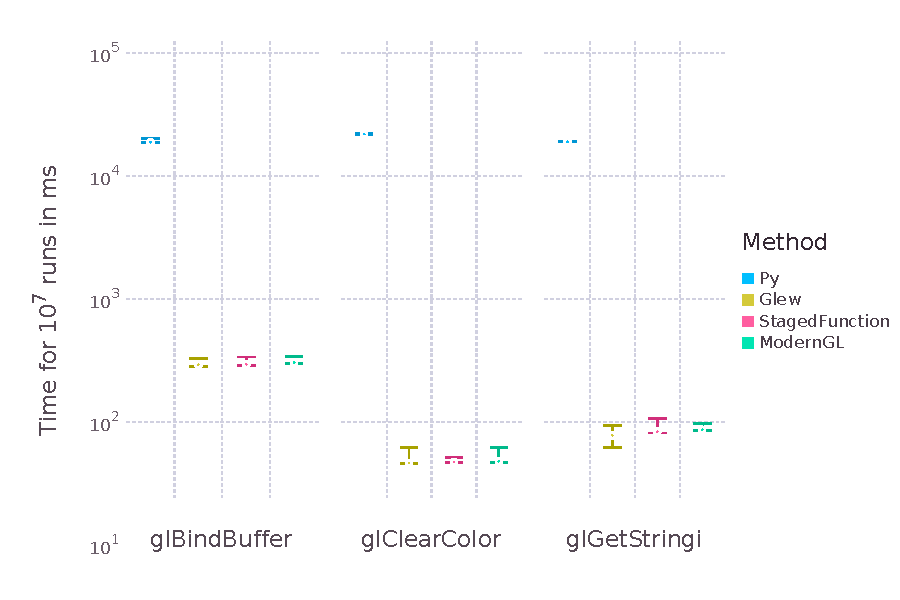
\includegraphics[width=0.9\linewidth]{graphics/glbench.pdf}
    \captionof{figure}[OpenGL Wrapper]{Different performance of OpenGL wrappers. The time for $10^7$ calls was measured 100 times for each function.}
    \label{fig:openglwrapper}
\end{minipage}
\begin{table}[htbp]
    \centering
    \begin{tabular}{l|c|c|c}
        \hline
        \textbf{Function}   & \textbf{Python}    & \textbf{Staged Function} & \textbf{ModernGL} \\
        \hline
        glBindBuffer        & 64.43              & 1.00 & 1.04 \\
        glClearColor        & 474.72             & 1.02 & 1.04 \\
        glStringi           & 244.44             & 1.07 & 1.1  \\
    \end{tabular}
    \captionof{table}[OGL Relative Speed]{Performance relative to C++ with Glew (slowdown, bigger is worse)}
    \label{table:relativespeedoglw}
\end{table}

In this chapter, ModernGL, GLEW and PyOpenGL will get benchmarked.
The procedure was, to call an OpenGL function $10^7$ times in a tight loop. The execution time of the loop got measured.
The results are plotted in figure \ref{fig:openglwrapper}.
ModernGL does pretty well compared to C++. Python comes out very slow, with being up to 470 times slower in the case of glClearColor.

In contrast, Julia offers nearly the same speed as calling an OpenGL functions from C++ as can be seen in the table \ref{table:relativespeedoglw}.
As all the OpenGL wrappers are pretty mature by now and bind to the same C library (the video driver), this should mainly be a C function call benchmark.
Python performs badly here, but it must be noted that there are a lot of different Python distributions and some promise to have better C interoperability.
As this benchmarks goal is to show that Julia’s \textit{ccall} interface is comparable to a C function call from inside C++, the python options have not been researched that thoroughly.
From this benchmark can be concluded, that Julia offers a solid basis for an OpenGL wrapper library.

\subsubsection{Reactive}

\begin{figure}
\centering
    \begin{minipage}{.5\textwidth}
        \centering
        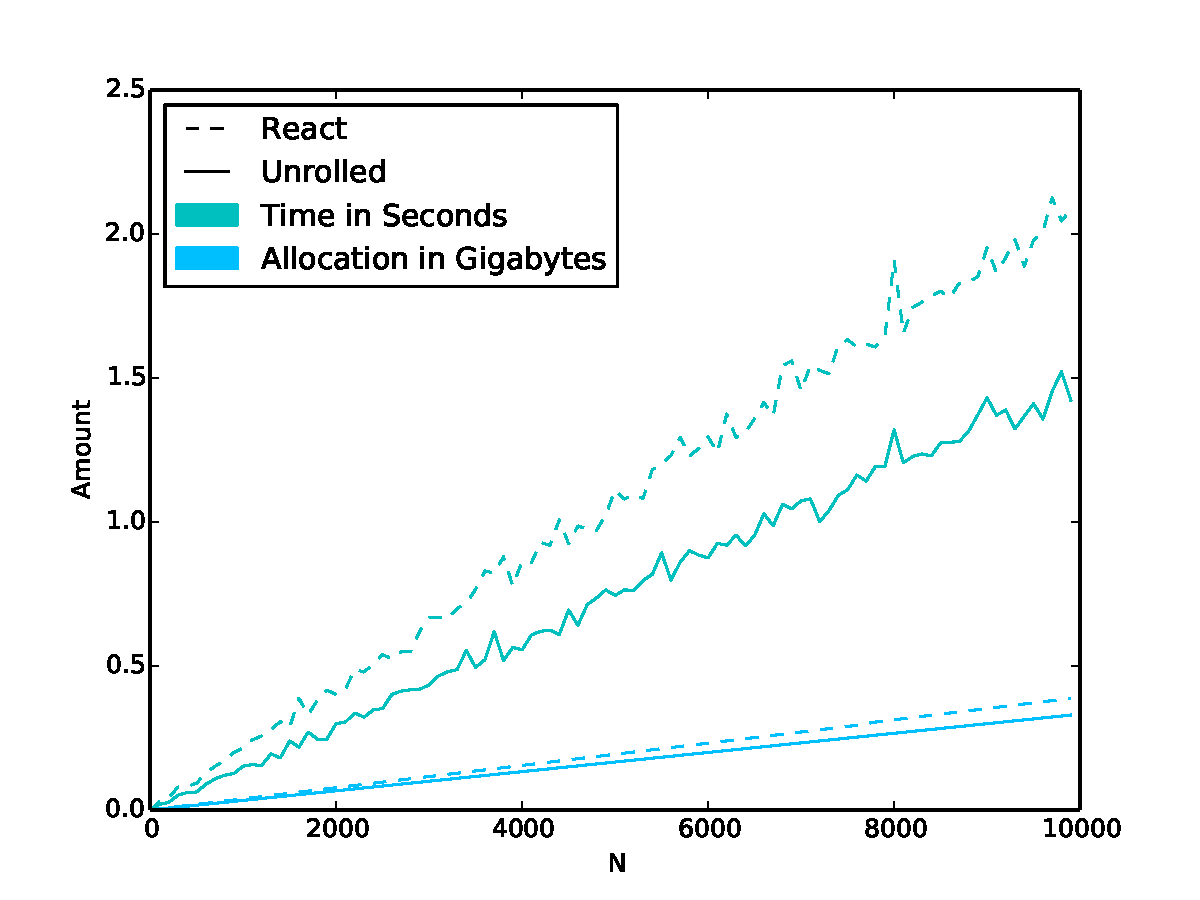
\includegraphics[width=0.9\textwidth]{graphics/react_bench_2.pdf}
        \captionof{figure}[Reactive 1]{Complicated graph, simple calculation}
        \label{fig:reactive1}
    \end{minipage}%
    \begin{minipage}{.5\textwidth}
        \centering
        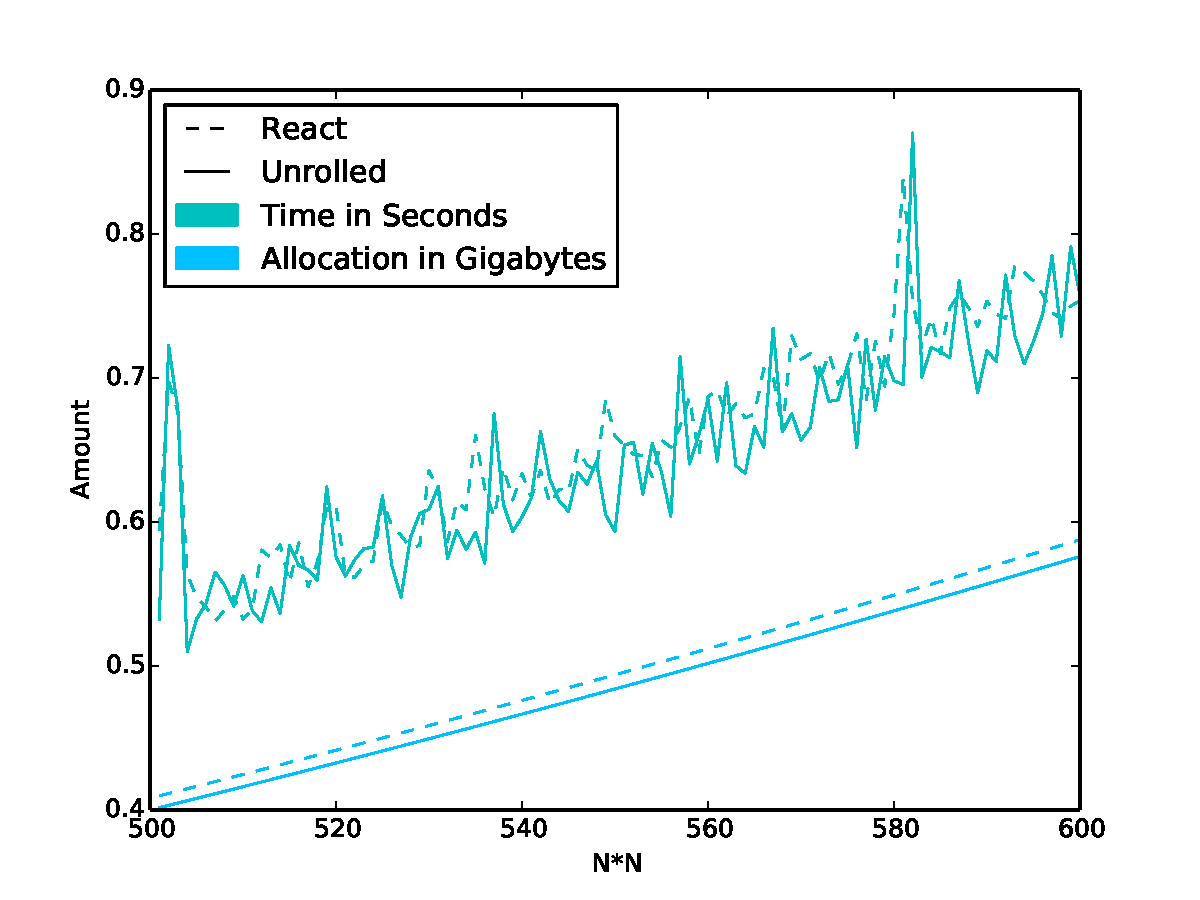
\includegraphics[width=0.9\textwidth]{graphics/react_bench_1.pdf}
        \captionof{figure}[Reactive 2]{High memory, simple event graph}
        \label{fig:reactive2}
    \end{minipage}
\end{figure}

It is relatively hard to benchmark the used event system in real world scenarios. To compare Rome's performance with different event systems, one would have to reimplement Romeo for every benchmark.
Using other visualization libraries as a baseline is also difficult, as it is hard to isolate the performance of the event system.
This is why we will compare an event graph from Reactive with its unrolled version.
For the unrolled version the functions from the callback-graph have been executed in the same order as the event graph would have without introducing any event system related overhead.
This way we can measure the overhead introduced by the event system.
Two code samples have been benchmarked, one simulating the operation needed for the camera and the other simulates animating a large array.
The first has low memory usage with a more complex event graph. The second has a straight forward event graph, but it must pass on a large array and needs to execute the callbacks on the array.

As can be seen in figure \ref{fig:reactive1}, small operations with a complex event graph have some noticeable overhead. Reactive is in this scenario about 1.45 times slower than the optimal version.
This does not come as a surprise as sorting and managing the graph structure adds some overhead.

The second scenario looks much better for Reactive. The performance difference is neglectable, making Reactive a good choice for creating signals with high memory throughput.

\subsubsection{3D Rendering Benchmark}

\begin{minipage}{\linewidth}
    \centering
    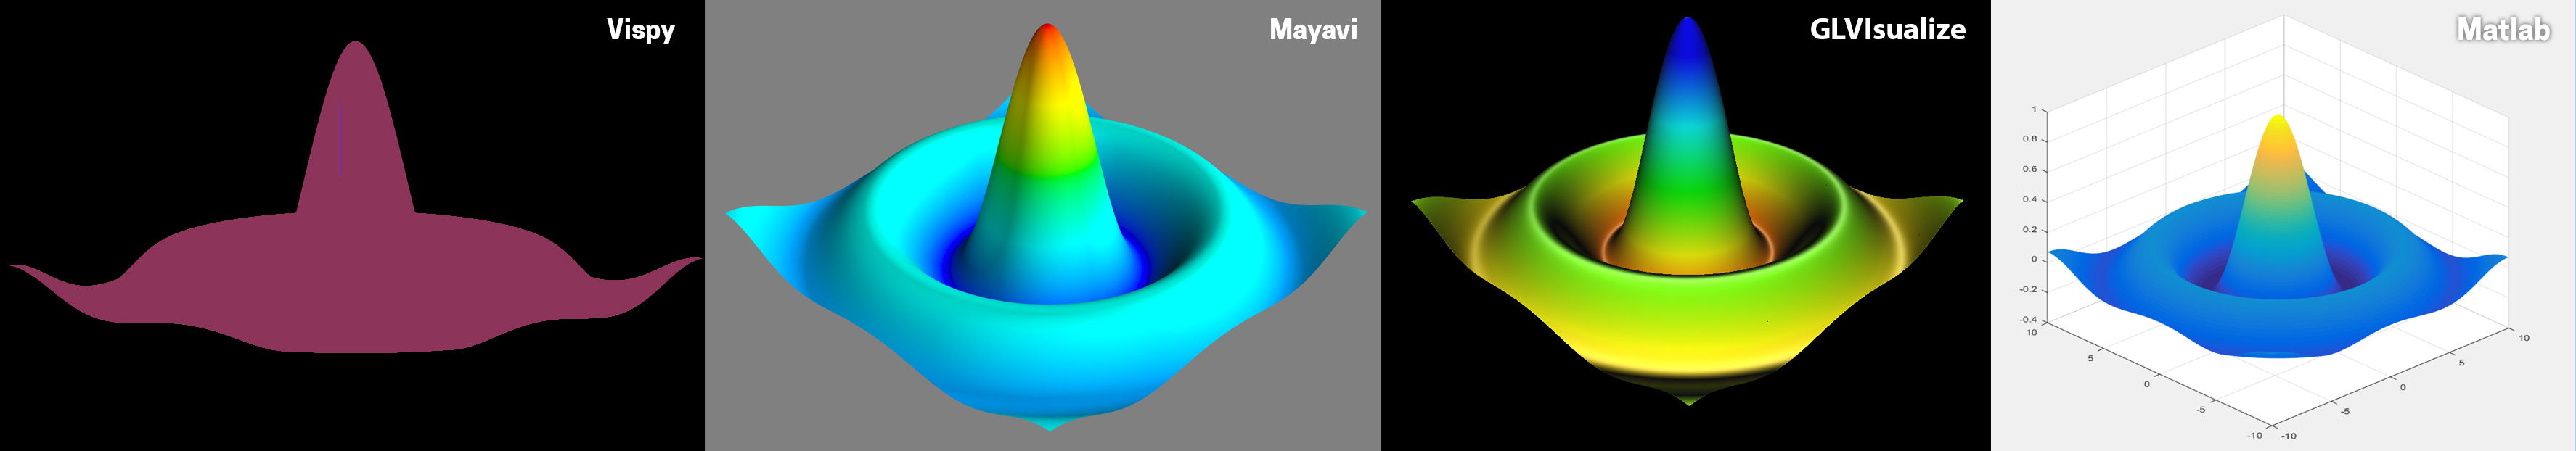
\includegraphics[width=\linewidth]{graphics/vispy_mayavi_romeo.jpg}
    \captionof{figure}[Benchmark]{Different visualizations of the same surface}
    \label{fig:reactive1}
\end{minipage}

The biggest problem with benchmarking the 3D rendering speed is, that there is no library which will allow to exactly reproduce similar conditions and measures. 
Additionally, without extensive knowledge of the library, it is difficult to foresee what gets benchmarked. 
Vispy shows, why it is difficult to rely on measurements like the frame rate. When you enable to measure the frame rate, it will show very low frame rates, as it only creates a new frame whenever the camera changes.
On the other side, Romeo has a fixed render loop, which renders as many frames as possible, leading to an entirely different amount of rendered frames per second. 
This is why it was decided, to use the threshold at which a similar 3D scene is still conceived as enjoyable and interactive. Usually the minimal amount of frames per second for perceiving movements as smooth is around 25.
So the benchmark was executed in the way, that the number regulating the complexity of the 3D scene was increased until one could not move the camera without stutters anymore. The last recorded pleasant threshold is then the result of the Benchmark.

The first benchmark is an animated and a still 3D surface plot. The libraries offering this functionality where Vispy, Mayavi and Matlab.

\begin{table}[htbp]
    \centering
    \begin{tabular}{l|l|l}
        \hline
        \textbf{Library} & \textbf{Still} & \textbf{Animated} \\
        \hline
        Vispy            & 300            & 80    \\
        Mayavi           & 800            & 150   \\
        Matlab           & 800            & 450   \\
        Romeo            & 900            & 600   \\
        \hline
        \hline
        Speed up Vispy   & 9x            & 56x   \\
        Speed up Mayavi  & 1.26x         & 16x   \\
        Speed up Matlab  & 1.26x         & 1.7x  \\
    \end{tabular}
    \captionof{table}[3D Benchmark]{3D surface created from a NxN matrix.}
    \label{table:relativespeedoglw}
\end{table}
Vispy had some issues, as the camera was never really smooth for the surface example. Also the normals were missing and there was no option to colorize the surface depending on the height.
It was decided to use the threshold of going from a little stutter to unpleasant stutters, making Vispy not completely fail this benchmark.
For Vispy, it was found that the normals were calculated on the CPU resulting in a major slow down\cite{VispyGithub}. The same can be expected from Mayavi, but Mayavi seems to be faster at calculating the normals.
There is not much information available on how Matlab renders their visualization, as it is closed source.

\begin{minipage}{\linewidth}
    \centering
    \includegraphics[width=\linewidth]{graphics/romeo_mayavi_particles.jpg}
    \captionof{figure}[Particles]{Rendered particles}
    \label{fig:reactive1}
\end{minipage}

The next benchmark is only between Romeo and Mayavi, as the other libraries did not offer a comparable solution. Matlab does not allow to use cubes as particle primitives and Vispy only had an example, where you needed to write your own shader, which can not be seen as a serious option. This is a benchmark for easy to use and high-level plotting libraries. We want to find out how well one can solve a problem with the tools the library has readily available.

\begin{table}[htbp]
    \centering
    \begin{tabular}{l|l|l}
        \hline
        \textbf{Library} & \textbf{Still}  & \textbf{Animated}  \\ 
        \hline
        Mayavi           & 90000           & 2500  \\
        Romeo            & 1000000         & 40000 \\
        \hline
        \hline
        Speed up         & 11x             & 16x \\
    \end{tabular}
    \captionof{table}[3D Benchmark]{Maximum number of particles that could be displayed without stutter.}
    \label{table:relativespeedoglw}
\end{table}

Romeo is an order of magnitude faster in this specific benchmark. This is most likely due to the fact that GLVisualize uses OpenGL's native instance rendering.
It can not get much faster than that. The next level of optimizations can be culling, which would only give an advantage at certain zoom levels.

\subsubsection{IJulia}

It was not possible to compare IJulia directly with Romeo, as the feature set for plotting is too different.

But there are certain factors, which indicate, that is hard to reach optimal performance with IJulia.
First of all, IJulia uses ZMQ to bridge the web interface with the Julia kernel.
ZMQ is a messaging system using different sockets for communication like inproc, IPC, TCP, TIPC and multicas.
While it is very fast at its task of sending messages, it can not compete with the native performance of staying inside one language.
This is not very important as long as there is not a lot of communication between Julia and the IPython kernel. This changes dramatically for animations, where big memory chunks have to be streamed to the rendering engine of the browser. It can be expected, that this will always be a weakness of IJulia.
On the other hand, GPU-accelerated rendering in a web browser is also limited.
It relies on WebGL, which offers only a subset of the OpenGL's functionality. While the execution speed of OpenGL can be expected to be similar, there are a lot of new techniques missing, which can speed up rendering. Also interoperability with  OpenCL and CUDA backends ranges from difficult to impossible. 
This makes it impossible to further accelerate massive parallel tasks.

Another benchmark was created to get a sense of what the current state of 3D rendering in IJulia is.
It is between Romeo and Compse3D, which was the only library found to be able to display 3D models created with Julia directly inside the IJulia notebook.
This benchmark is not entirely fair, as Compose3D is just a very rough prototype so far. 
But there seem to be no other library in which you can easily create and display interactive 3D graphics in the IJulia or IPython notebook. 
This benchmark creates a Sierpinski gasket and Compose3D displays it in the IJulia notebook while Romeo displays it natively in a window.

\begin{minipage}{\linewidth}
    \centering
    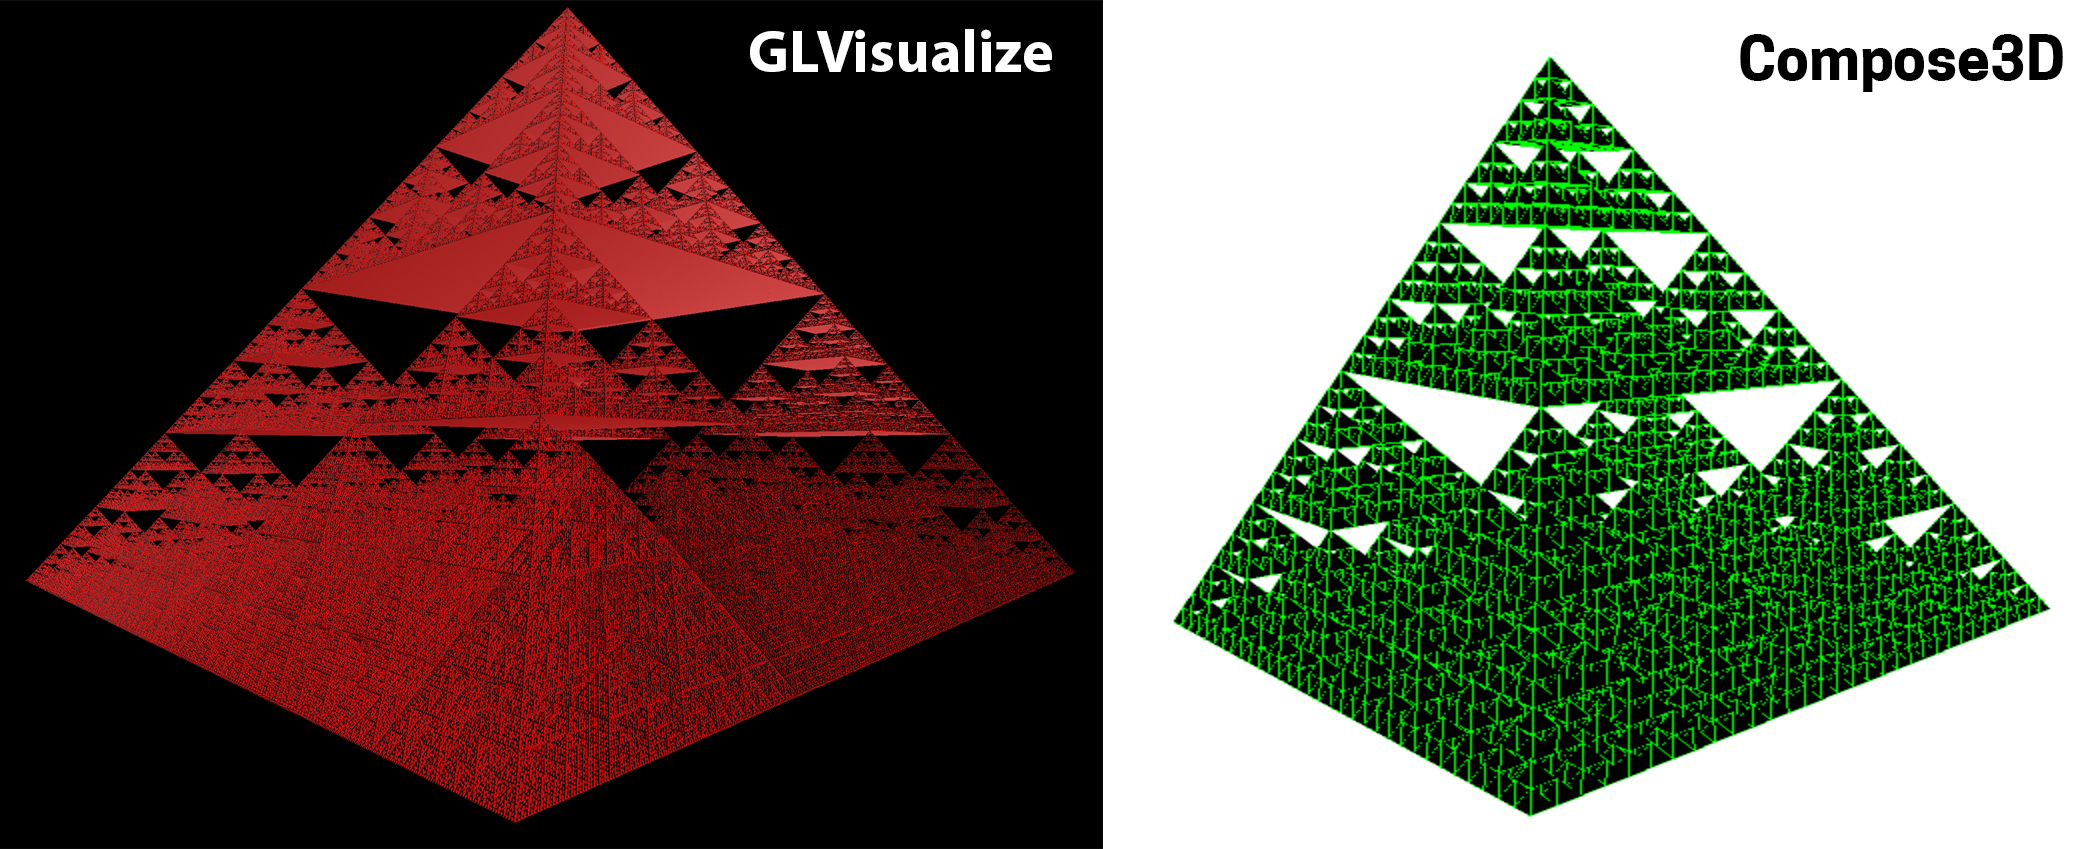
\includegraphics[width=\linewidth]{graphics/sierpinsky.jpg}
    \captionof{figure}[Sierpinski]{Sierpinski pyramid in 3D}
    \label{fig:reactive1}
\end{minipage}
\begin{table}[htbp]
    \centering
    \begin{tabular}{l|l}
        \hline
        \textbf{Library} & \textbf{Still}\\ 
        \hline
        Compose3D        & 15625         \\
        Romeo            & 1953125       \\
        \hline
        \hline
        Speed up         & 125x          \\
    \end{tabular}
    \captionof{table}[3D Benchmark]{Maximum number of pyramids that could be displayed without stutter.}
    \label{table:relativespeedoglw}
\end{table}

Romeo is an order of magnitude faster. This can change in the future when Compose3D matures.
But one needs to notice, that Romeo utilizes OpenGL's instancing to gain this speed. Native instancing is not yet available in WebGL, which means that this optimization will not be available for the IPython notebook in the near future.

\subsection{Extensibility Analysis}

The modular design of Romeo has proven to be effective and the goal of reusability has already proven itself.
Most of the created modules are used independently by different people.
GLVisualize is used by myself for two packages, namely GLPlot, a scientific plotting package for Julia and a 3D printing startup uses it for rendering their 3D models. [sources]
It got forked by several users to create their own dynamic visualization packages.
The same applies for ModernGL and GLAbstraction. Most other used packages are at least used by one other project.
This indicates, that the abstraction and modularity is well designed, so that all the modules can be used alone.

The only exception is GLWindow, which has been used just indirectly through the other packages. 
This can mean three things.
Firstly, it is badly abstracted and does not cleanly wrap one use case.
Secondly, it can be that the use case is not entirely clear to other people, which would not be a big surprise considering the minimal amount of documentation for GLWindow.
And finally, considering the small group of people developing graphics for Julia, it could be that they simply do not need the lower level functionality of GLWindow and instead rely on the other written packages that use GLWindow.

From further analyzing the Github repository written for this thesis, one can find out that there is a general lack of documentation.
This hinders people from contributing and using the packages. This definitely needs to improve in the future to fully unfold the potential of the packages.

The implementation in just one language has been achieved by choice. 
There are only a few exceptions, like the kernel code for OpenGL shaders, which currently can not be written in Julia. 
Julia programmers that use Romeo can extend Romeo with Julia and immediately see their results without complicated compilations.
This together with the speed is one of the main achievements compared to other libraries offering similar functionality, like IJulia, Mayavi and Matlab.
To further proof this point I will analyze the mentioned software in more detail.
The language usage statistics and necessary tools needed in order to extend the software will be the main focus of the analysis.
One needs to note, that the usage statistic of languages is just a weak indicator for the extendability of a software.
Using different languages for one project can make sense if the project has different domains where domain specific languages give an advantage. 
As this still means that one needs to be fluent in all used languages, this still introduces complexity, but it is at least justified complexity.
This chapter will only discuss the complexity introduced by languages, which are only needed for compatibility with other libraries or because the main language is too slow. 
This is something, which should ideally be avoided.
For this analysis, a complex case like the integration of OpenCL into the visualization pipeline will be used as an example.


\subsubsection{Romeo}

\begin{table}[htbp]
    \centering
    \begin{tabular}{l|l|l|l|l}
        \hline
        \textbf{Language} & \textbf{files}    &   \textbf{blank}   &   \textbf{comment}    &  \textbf{code}\\
        \hline
        Julia  &  101   &    1231 &   281  &  5499\\
        C       &   28  &   273   &    114 &  1090\\
        \hline
        SUM: & 132  &  1504  &     395    &   6641\\
        \hline
    \end{tabular}
    \captionof{table}[Romeos Stack]]{Julia Repositories}
    \label{table:romeo_loc}
\end{table}

In GLVisualize every customization can be done from within Julia.
Everything like OpenGL context handles and OpenGL buffers are accessible.
One can implement even advanced features like OpenCL context with GLvisualize and Julia.
This is made especially easy, as all visualization functions are defined on the GPU objects. So if one has a GPU array from some other calculation, one can directly visualize it without additional memory transfers.
But even in the worst case, if the whole architecture is not well fitted for the task, reimplementing large parts would not be difficult as there are only 6641 lines of code which are mostly written in Julia (see table \ref{romeo_loc}.
If it comes even worse and the language itself has to be modified for the features, this will pose no problem as Julia is open source.
This allows to implement advanced features like running Julia code directly on the \ac{GPU}.


\subsubsection{IJulia}


\begin{table}[htbp]
    \centering
    \begin{tabular}{l|l}
        \hline
        \textbf{Software} & \textbf{languages used}\\
        \hline
        IPython     & Python 78.5\% JavaScript:15.1\% HTML 5.0\% Other 1.4\%\\
        Three.js:   & JavaScript 62.4\% HTML 26.4\% Python 6.9\% C++ 1.9\% C 1.3\% GLSL 0.6\%\\
        D3:         & JavaScript 95.6\% CSS 4.3\%\\
        \hline
    \end{tabular}
    \captionof{table}[IJulia Stack]]{Technologies used in IJulia. Statistics taken from Github}
    \label{table:ijuliastack}
\end{table}

IJulia is written in Julia and relies on ZMQ and IPython.
ZMQ is written in C++ to make it as fast as possible.
IPython uses multiple JavaScript rendering backends like Three.js and D3.
The graphical notebooks are running inside a browser, which adds another complex technology stack.
One the plus side, most technologies used are open source, which in theory would allow for customizations of the entire stack.

IPython is written in Python, so using IPython from Julia forces you to already use two similar languages.
JavaScript, CSS and HTML are only needed to render graphics inside the browser. CSS and HTML can be seen as a domain specific languages for creating \ac{GUI}s, so while introducing yet another language, they bring the value of easy \ac{GUI} creation.
C++ offers similar functionality to JavaScript and Python, so it can be assumed it was used for speed and interoperability with other C++ libraries.
So IJulia builds upon a very heterogeneous technology stack, making it difficult to add advanced features.
From inside Julia, there are no handles to the actual rendering process. These are written in other languages, mainly JavaScript and Python.
Further rendering extensions which do not rely on combining functions from other libraries are only available by emiting HTML and Javascript code from Julia.
While modern Browsers seem to offer context sharing between WebGL and WebCL (the counter parts for OpenGL and OpenCL), it must be done via JavaScript.

All in all, from within Julia there are little options to implement completely new, advanced rendering features.



\subsubsection{Mayavi and VTK}
\begin{table}[htbp]
    \centering
    \begin{tabular}{l|l|l|l|l}
        \hline
        \textbf{Language} &    \textbf{files} &    \textbf{blank} &  \textbf{comment} &  \textbf{code}\\
        \hline
        Python          &               541      &    15430     &    24414   &       47673\\
        C               &                 1      &     202      &      354   &      1913\\
        make            &                 1      &       15     &         4  &        91\\
        Cython          &                 1      &       25     &        45  &        72\\
        Fortran 77      &                 1      &       21     &        28  &        60\\
        HTML            &                 1      &       10     &         0  &        54\\
        YAML            &                 1      &        0     &        5   &       31\\
        \hline
        SUM:            &               547       &   15703     &     24850  &       49894\\
        \hline
        \end{tabular}
    \captionof{table}[Mayavi]]{Mayavi language statistik}
    \label{table:mayavistatistic}
\end{table}

Mayavi itself is mostly written in Python, which amounts to an impressive 49,894 lines of code. This is quite a lot, considering that this does not include rendering code, which is done in VTK.
As can be seen in table \ref{table:VTKStatistic}, VTK alone amounts to a total of 2,812,005 lines of code written in approximately 27 languages. 
So the main problem for extending VTK and Mayavi's core will be its complexity. If you're willing to switch to C++, VTK will allow you to implement any advanced feature. From inside Mayavi and Python, one will have problems with the accessing the underlying rendering core of VTK and probably also performance problems with Python.


\subsubsection{Matlab}

Matlab is closed source, which makes the core of Matlab impossible to extend by the user. 
To extend functionality which needs to modify the language or the core library one will have to ask the mathworks to do that for you.
This is why Matlab relies on a plug-in architecture which enables developers to write closed or open source plug-ins for Matlab. 
Simple packages can be written in Matlab itself and imported into a project.
This is not an option for performance critical plug-ins though, as the Matlab language is too slow.
So something like a 3D visualization library should not be written in pure Matlab code.
For that a mex plug-in is best fitted, which is Matlab's way of letting one write C/C++ plug-ins.
It is a very simple process of including a Matlab header file into the C/C++ source, which can then be compiled with Matlab.
The header file holds types, which can be used to make the C/C++ functions work with Matlab's native types.
It also holds the \textit{mexFunction} macro, which needs to be used in order to make the function callable from Matlab.
So it seems to be fairly easy to integrate C/C++ code, but it also defies the purpose of writing in a scientific programming language.
But worst of all, the visualization core itself is not extendable. This means as soon as you want to do something more advanced, you need to start from scratch, or call out to some third party library.


\subsection{Usability Analysis}
%Consistency and ease of use of programming API in GLVisualize+GLAbstraction and Romeo.
%Short comment about the \ac{GUI}
Doing a broad user survey or similar methods was out of scope for this thesis.
This is why the usability study has to be done analytically.
There are different aspects which can be analyzed. For example, how many function names need to be remembered, how easy they are memorized, if they expose the wanted functionality and how difficult it is to look up unknown functionality.
The main user facing \ac{API}, namely GLVisualizes will be analyzed for this thesis. 
The named aspects will be analyzed together with feedback from Github.

\subsubsection{GLVisualize}

GLVisulize has a very simple API, as it offers only four functions: \textit{visualize}, \textit{visualize\_defaults} and \textit{edit}.
There are also the functions bounce and loop, which offers a simplification for creating periodic signals.
These functions might get moved into Reactive, though.
So for GLVisualize, only very few function names have to be remembered.
The question is, if this simple interface still allows people to create the visualization they want.
At closer inspection one can see, that visualize is overloaded 67 Julia types, with each of these methods having a set of keyword arguments which enable further customization.
These can introduce drastic changes. The particle visualization for example can take any mesh as a primitive. This allows a level of customization, which was not possible in the other examined packages.
Also, most of the functions take either a data type, or a signal of that data type.
This makes it very intuitive to animate your data. 
In contrast, in order to setup the animation for the other packages, it took quite some time to find out how to update values of an existing visualization. This is acceptable, as it might take quite some time to find out that Romeo uses signals and how to work with signals.
But when this is found out, Romeo functions in the same, consistent way. Signals add a fourth dimension to any parameter or data you would like to visualize, making the usage principle consistent across the different visualizations.

For the other packages though, one needs to find out the names of the data for every visualization type in order to access and update them. Some attributes can not be animated, making the API even less consistent.

So for Romeo one can achieve anything by bringing the data into the right format.
Problems arise, if this can not be done easily or the format is not intuitive for the programmer.
To be fair, you will have this problem with every kind of visualization API. 
In the end the only difference is, how easy it was to do the data transformations. 
Let us examine an example, where GLVisualize often will not allow to directly call visualize on the data.
There is only a method for visualizing a Mesh, but not for a vertex list plus a face list. 
If one works with mesh data, one will often handle the face and vertex list in isolation.
So an API that offers a function like \texttt{visualize\_mesh(x::VertexList, y::FaceList)} will be more straightforward for the programmer.
This is actually the standard way of displaying a mesh in most scientific plotting packages. This has become one of the most occurring questions on Github, even though that there are usage examples for displaying a mesh.
So diverting from standard plotting interfaces might be the biggest usability issue for GLVisualize.
This is not necessarily an issue. 
It is quite easy to offer a compatibility package, which defines functions like \texttt{
visualize\_mesh(facelist, vertexlist) = visualize(Mesh(facelist, vertexlist))}.
As GLVisulize should stay as close to the principle of only having one function name, this should be moved to other interface only packages, though.

The functionality of GLVisualize is easy to explore. There are only three function to be remembered. From there it is easy to find out how they work. First, you can just call visualize on your data and see if the default is already sufficient. If not, you can call visualize_defaults on the data, to find out what kind of default parameters there are, which can then be tweaked. As an alternative, one can edit every parameter of the visualization on the spot via the widgets. 
If that is not enough, a list of the data types that can be visualized can be queried with Julia in builds. 
In the same way one could also query help for the visualization type.


